\documentclass{article}
\usepackage[utf8]{inputenc}
\title{video 1: THE NULL HYPOTHESIS AND THE P VALUE}
\author{wbg231 }
\date{December 2022}
\newcommand{\R}{$\mathbb{R}$}
\newcommand{\B}{$\beta$}
\newcommand{\A}{$\alpha$}
\newcommand{\D}{\Delta}

\newcommand{\avector}[2]{(#1_2,\ldots,#1_{#2})}
\newcommand{\makedef}[2]{$\textbf{#1}$:#2 }
\usepackage{tikz,graphicx,hyperref,amsmath,amsfonts,amscd,amssymb,bm,cite,epsfig,epsf,url}

\begin{document}

\maketitle

\section*{introduction}
\begin{itemize}
\item \href{https://www.youtube.com/watch?v=d0jC1pQN6P8&list=PLBEf5mJtE6KuZ5NBQMuWIMsiOOrV9ibzm&index=78}{video link}
\item we are going to introduce concepts in hypothesis testing including the null hypothesis test stat and p-value 
\item the goal of hypothesis testing is to see whether the data we observe supports a conjecture, we do this by assuming the patterns in this data are caused by pattern, and we see how likely the data is to be true under random chance. 
\subsection{null hypothesis}
\item contradicts the conjecture, ie devils advocate. 
\item for instance, it could be the idea that the die is fair. 
\item our original conjecture is called the \textbf{alternative hypothesis }
\subsection{test statistic}
\item in order to evaluate the null hypothesis we need to look at the data, using a test stat that is a function of that data associated to our alternative hypothesis 
\item the test stat should Be large if our null hypothesis does not hold 
\item in the case of the die example, it would be the number of 3. 
\item so a large number of 3s is evidenced against the null hypothesis. 
\subsection{die example}
\item alternative hypothesis $P(\textbf{roll three})> \frac{1}{6}$
\item null hypothesis $P(\textbf{roll three})=\frac{1}{6}$
\item test stat number of 3s
\item suppose we see 18 3s out of 60 rolls is this unlikely under the null hypothesis 
\item in short yeah it is unlikely, but no that is not the end of the story. 
\item we have committed a sin in the sense that we made our hypothesis after looking at the data 
\subsection{licence plates}
\item suppose you are walking down the street in NYC and see a certain licence plate, and your Friend says, "wow isn't is surprising we saw this number when there are so many combinations" no it is not astounding since, we did not specifies the number before hand it is equivalent to seeing any licence plate number
\item so if we fix the number before hand it would be amazing, but we did not so it is not amazing 
\item unless we fix the hypothesis before hand we do not know what to look at to find evidence of our null
\subsection{hypothesis testing}
\item step 1: decide the null hypothesis (with out looking at the data)
\item step 2: chose test stat with out looking At data 
\item step 3: evaluate the test stat on the data a
\tem step 4: determine how likely it is under the null hypothesis, this requires modeling the distribution of the test stat under the null 
\section{parametric testing}
\subsection{parametric testing}
\item we make the assumption that the test stat has a distribution that depends on a number of parameters $\theta$
\item \textbf{simple null hypothesis}, parameters equal singe value $\theta= \theta_{null}$
\item \textbf{composite null hypothesis}, parameters equal singe value $\theta\in \Theta_{null}$
\subsection{die roll}
\item assumption rolls are independent 
\item call the probability of rolling a three $\theta$
\item test stat the number of three out of 100 new rolls (we have not seen at this point) 
\item distribution if we think that the probability of rolling a three is $\theta$ and that the probability of each roll is independent then the likelihood of rolling a certain number of 3s is binomial $P(k,\theta)=\begin{pmatrix}n\\k\end{pmatrix}(\theta)^{k}(1-\theta)^{n-k}$ with n=100
\item lets call our simple null $\theta=\theta_{null}=\frac{1}{6}$ (we could also chose a comprise null hypothesis of the form $\theta\in \Theta_{null}=[0,\frac{1}{6}]$
 \item observed static  21 3's seen. 
 \item the question is now how likely is it to observe 21 or more 3's under the null hypothesis. ( we use the or more as well since, we would consider more extreme examples also as evidence against the null) 
 \subsection{p - value}
 \item \textbf{p- value}- the likelihood of observing a test statistic that is larger than or equal to what we saw under the null hypothesis. 
 \subsection{simple null}
 \itme under a simple null hypothesis $\theta=\theta_{null}$
 \item \textbf{p-value function} $$pv(t)=P(\Tilde{t}_{\theta_{null}\geq t})$$
\item p value of our data is $pv(t_{data})$
\subsection{die rolls }
\item we want to compute the p-value function for our die roll 
\item $pv(t)=P(\Tilde{t}_{\theta_{null}\geq t})= \Sigma_{i=t}^{100}p(i,\theta)=\Sigma_{i=t}^{100}\begin{pmatrix}100\\i\end{pmatrix}(\frac{1}{6})^{i}(\frac{5}{6})^{100-i}$under our assumptions 
\item so if we plug in our $t__{data}=21$ we can see that $pv(t_{data})=.15$ ie there is a 15\% chance that is due to random chance 
\item 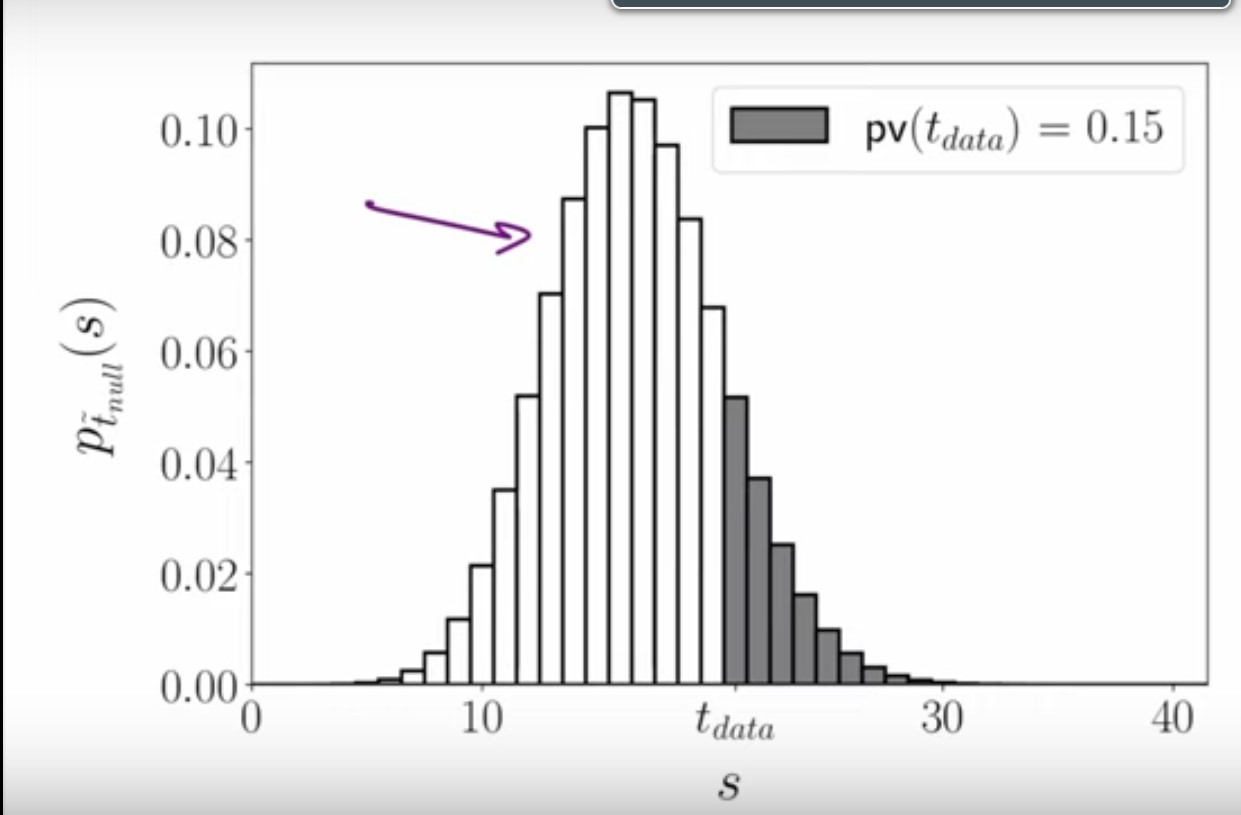
\includegraphics[width=10cm]{notes/week_6/vidio 1: THE NULL HYPOTHESIS AND THE P VALUE/immages/v1_1.jpg}
\item so that is what our distribution of test stats under the null looks like looks like, and the sum of the pmf from 21-100
\item here is what our p-value function looks like, it is falling in the number of 3's we observe in our data 
\item 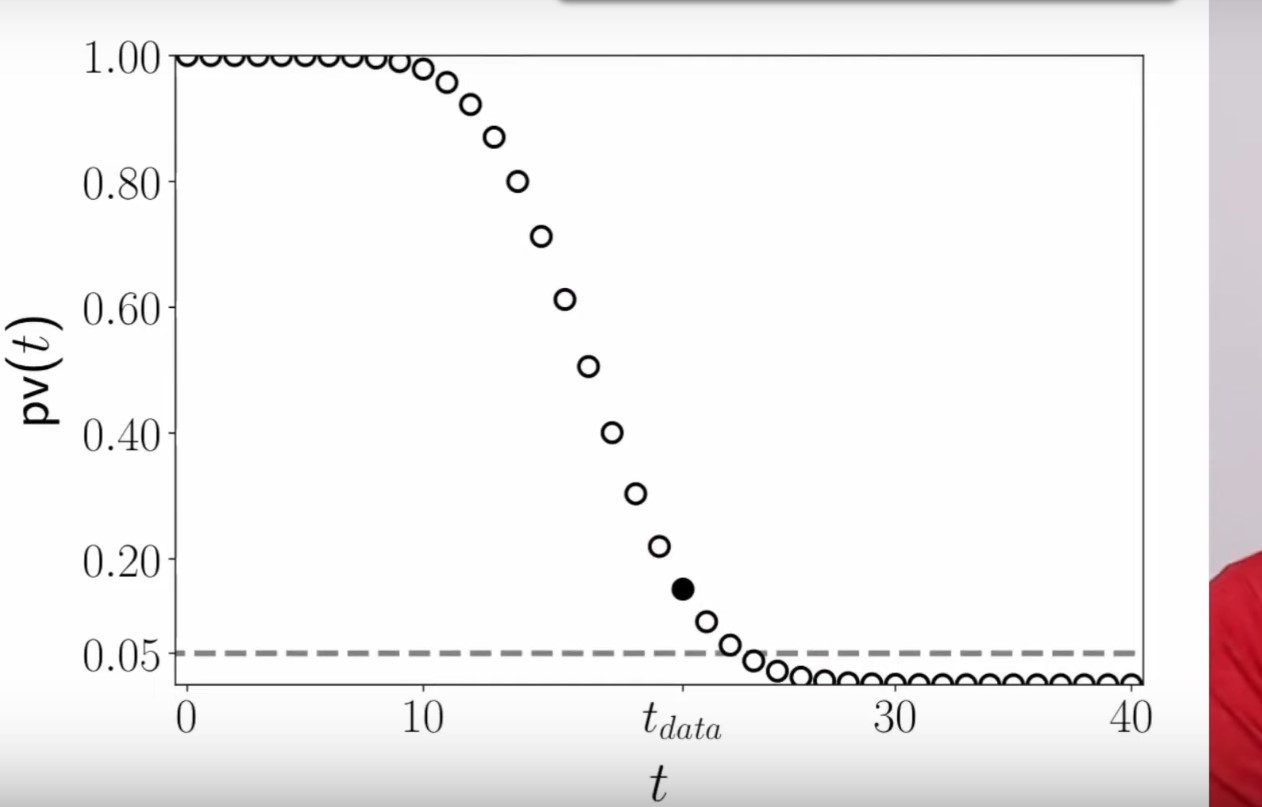
\includegraphics[width=10cm]{notes/week_6/vidio 1: THE NULL HYPOTHESIS AND THE P VALUE/immages/v1_2.jpg}
\item this is kind of in the middle
\subsection{composite null hypothesis}
\item in the case of a composite null hypothesis $\thea\in \Theta_{null}=[0,\frac{1}{6}]$
\item we define our p value function as $$pv(t)=sup_{\theta\in \Theta_{null}}P(\Tilde{t}_{\theta}\geq t)$$
\item so that is out of all the $\theta$ we are thickening of, what is the $\theat$ that gives us the max probability of seeing this number of 3's or more
\item then the p value of our data remains $pv(t_{data})$
\item so in our example that would be $pv(t)=sup_{0\leq \theta\leq \frac{1}{6}}P(\Tilde{t}_{\theta}\geq t)=\\sup_{0\leq \theta\leq \frac{1}{6}}\Sigma_{i=1}^{t}\begin{pmatrix}
100\\i    
\end{pmatrix}\theta^{i}(1-\theta)^{100-i}=\Sigma_{i=t}^{100}\begin{pmatrix}100\\i\end{pmatrix}(\frac{1}{6})^{i}(\frac{5}{6})^{100-i}$
\item in this case the composite changes nothing as the highest value of $\theta$ is the largest probability that is $\frac{1}{6}$ which was what we chose for our simple null
\subsection{p-value}
\item it is temping to interpret this as the probability that the die is fair ie $\theta=\frac{1}{6}$ is .15 but \textbf{that is false}
\item we have modeled this problem from a frequentest point of view so there is nothing random. $\theta$ is deterministic. (this is similar to the problem interesting confidence intervals)
\item \textbf{correct interpretation} if 
the null hypothesis is true than the probability of observing more than 21 3's out of 100 rolls is 0.15
\section{statistical significance}
\item  we reject the null hypothesis when p-value $\leq \alpha$
\item this gauntness that the probability of a false positive $\leq \alpha$
\item a false positive (type 1 error) is a case where the null is true but we reject it. 
\subsection{die roll}
\item if we set $\alpha=.05$ and we observe a p value of .15 then we fail to reject the null
\item this does not mean the die is fair, it just means we do not have enough evidence to say it is unfair
\item it is a very strict frame work, because there are a lot of cases we can not say anything. we are mainly focoused on saying if we found something it is really there. 

\end{itemize}

\end{document}
